\documentclass[11pt,letterpaper]{article}
% === graphic packages ===
\usepackage{epsf,graphicx,psfrag}
% === bibliography package ===
\usepackage{natbib}
% === margin and formatting ===
\usepackage{setspace}
%\usepackage{palatino}[1]
%\usepackage[T1]{fontenc}
%\usepackage{palatino}
%\renewcommand{\familydefault}{cmss}
%\usepackage{cmbright}
%\usepackage[T1]{fontenc}
%\usepackage{arev}
%\usepackage[LGR,T1]{fontenc} %% LGR encoding is needed for loading the package gfsneohellenic
%\usepackage[default]{gfsneohellenic}
%\usepackage{times}
\usepackage{fullpage}
\usepackage{color}
\usepackage{endnotes}
% === math packages ===
\usepackage[reqno]{amsmath}
%\usepackage[pdftex]{hyperref}
\usepackage{amsthm}
\usepackage{amssymb,enumerate}
\usepackage[all]{xy}
\usepackage{lscape}
\usepackage[compact]{titlesec}
%\newtheorem{lem} {Lemma}
%\newtheorem{prop}{Proposition}
%\newtheorem{thm}{Theorem}
%\newtheorem{defn}{Definition}
%\newtheorem{cor}{Corollary}
%\newtheorem{obs}{Observation}
 \numberwithin{equation}{section}
% === dcolumn package ===
\usepackage{dcolumn}
\newcolumntype{.}{D{.}{.}{-1}}
\newcolumntype{d}[1]{D{.}{.}{#1}}
% === additional packages ===
\usepackage{url}
\newcommand{\makebrace}[1]{\left\{#1 \right \} }
\newcommand{\determinant}[1]{\left | #1 \right | }
\title{Mathematical Foundations Practice Questions}
\date{March 6, 2017}
\begin{document}
\maketitle
\subsection*{Instructions}
These are practice questions:
\begin{enumerate}[I]
\item \textsc{Probability and Mathematical Logic }
\begin{enumerate}[1)]
\item Comment on the veracity of the following statements in one sentence:
\begin{enumerate}
\item A correlation coefficient of zero between two variables indicates that they are independent.
\item[A)] FALSE.  Two variables can be uncorrelated but not independent if, for example, they are not linearly dependent.
\item For events A and B, $P(A\cap B) < P(A)+P(B)-1$
\item[A)] FALSE.   This would imply that 
$$1< P(A)+P(B)-P(A\cap B) $$
but $P(A)+P(B)-P(A\cap B)=(A\cup B)\leq 1$, so it is false.\\

In fact, $1 \geq P(A\cup B) =P(A)+P(B) - P(A\cap B)$  so $P(A\cap B) + 1 \geq P(A)+P(B) $, therefore $P(A\cap B) \geq P(A)+P(B) - 1$
\item E(XY)=E(X)E(Y)
\item[A)] FALSE.  Only if X and Y are independent is this true.

\item To show that events $A$, $B$, and $C$ are independent, it is sufficient to show that $$P(A\cap B \cap C)=P(A)P(B)P(C)$$
\item[A)] FALSE.  You must also show that the pairs are independent

\end{enumerate}
\pagebreak
\item Let $A$ and $B$ be two independent events with $P(A)= .4$ and $P(A\cup B)=.64$.  What is $P(B)$?
\item[A)] 
$$P(A\cup B)=P(A)+P(B)-P(A\cap B)$$
, by independence, 
$$P(A\cup B)=P(A)+P(B)-P(A)*P(B)$$
$$.64=.4+P(B)-.4*P(B)$$
$$.64=.4+(.6)*P(B)$$
$$.24/.6=P(B)=.4$$


\item  If E and F are independent, are $E^c$ and $F^c$ independent?  
\item[A)] Yes.
\end{enumerate}



\item \textsc{Word problems}  
\begin{enumerate}
\item 20\% of people in a town usually vote for the Green Party. 30\% of the people in town are unhappy with the current government. But 80\% of the people who usually vote for the Green Party are unhappy with the current Government. If you know that your neighbor is not happy with the current government, what is the probability that she usually votes for the Green Party?

ANSWER: P(Green$|$unhappy)=P(unhappy$|$Green)*P(Green)/P(unhappy)= $\frac{.8*.2}{.3}=.53$



\item In a congressional election, the incumbent is a Republican (R). Three Democrats (D1, D2 and D3) are seeking the Democratic nomination. The probabilities that they win are, respectively, 0.35, 0.40 and 0.25. Furthermore, polls show that R would have a 0.40 probability of defeating D1 in the general election, 0.35 probability of defeating D2, and a 0.60 probability of defeating D3. Assuming all these estimates to be accurate, what are the chances that the incumbent retains his seat?

ANSWER: Uuse Law of total probability:\\

 P(RETAIN)=P(RETAIN$|$D1)*P(D1)+P(RETAIN$|$D2)*P(D2)+P(RETAIN$|$D3)*P(D3)= .4*.35+.35*.40+.6*.25=.43
\end{enumerate}
\pagebreak
\item \textsc{Distributions} 
\begin{enumerate}

\item Suppose that 
$$f_{XY}(x,y)=\begin{cases} 6e^{-2x-3y} & \text{for } 0< x \text{ and }0<y \\ \\ 0 &\text{else}
\end{cases}$$
\begin{enumerate}[1)]
\item  Verify that $f_{XY}(x,y$) is a pdf. 
\item[A)] It is always positive and $\int_0^\infty \int_0^\infty 6e^{-2x-3y} dx dy=\int_0^\infty 0 +3e^{-2*0-3y} dy =0+ e^{-3*0}=1$ so it is a pdf.
\item Are X and Y independent?
\item[A)] They are independent iff $f_{XY}(x,y)=f_X(x)*f_Y(y)$  $f_Y= 3e^{-3y}$ $f_X=2e^{-2x}$.   $3e^{-3y}*2e^{-2x}=6e^{-2x-3y}$, so yes, they are.

\item What is $f_{y|x}(y)$?
\item[A)] $f_{y|x}(y)=f_y(y)$ because they are independent. $3e^{-3y}$
\end{enumerate}
\pagebreak
\item A pizza restaurant promises to deliver your order to the table within 10 minutes. Let Y be the time between ordering and the arrival of the pizza and suppose that the pdf of Y is:
$$f_{Y}(y)=\begin{cases} ky^2 & \text{for } 0<y< 10\\ 0 &\text{else}\end{cases}$$
\begin{enumerate}[1)]
\item Determine the value of k.  
\item[A)] $\int_0^{10} ky^2dy=1$ by the fact that this is a pdf.  So $k/3*10^3=1$, and $k=3/1000$
\item What is $Var(Y)$?
\item[A)] $Var(Y)= E(Y^2)-[E(Y)]^2$.  So $\int_0^{10} y^2 \frac{3}{1000}y^2dy-[\int_0^{10} y \frac{3}{1000}y^2dy]^2$

$$\int_0^{10} y^2 \frac{3}{1000}y^2dy=\frac{3}{5000}y^5|_0^{10}=\frac{3}{5000}10^5=600$$

$$\int_0^{10} y \frac{3}{1000}y^2dy=\frac{3}{4000}y^4|_0^{10}=\frac{3}{4000}10^4=7.5$$

$600-7.5=592.5$

\item  Find the cdf of Y and graph it.
CDF :  $\frac{1}{1000}y^3$

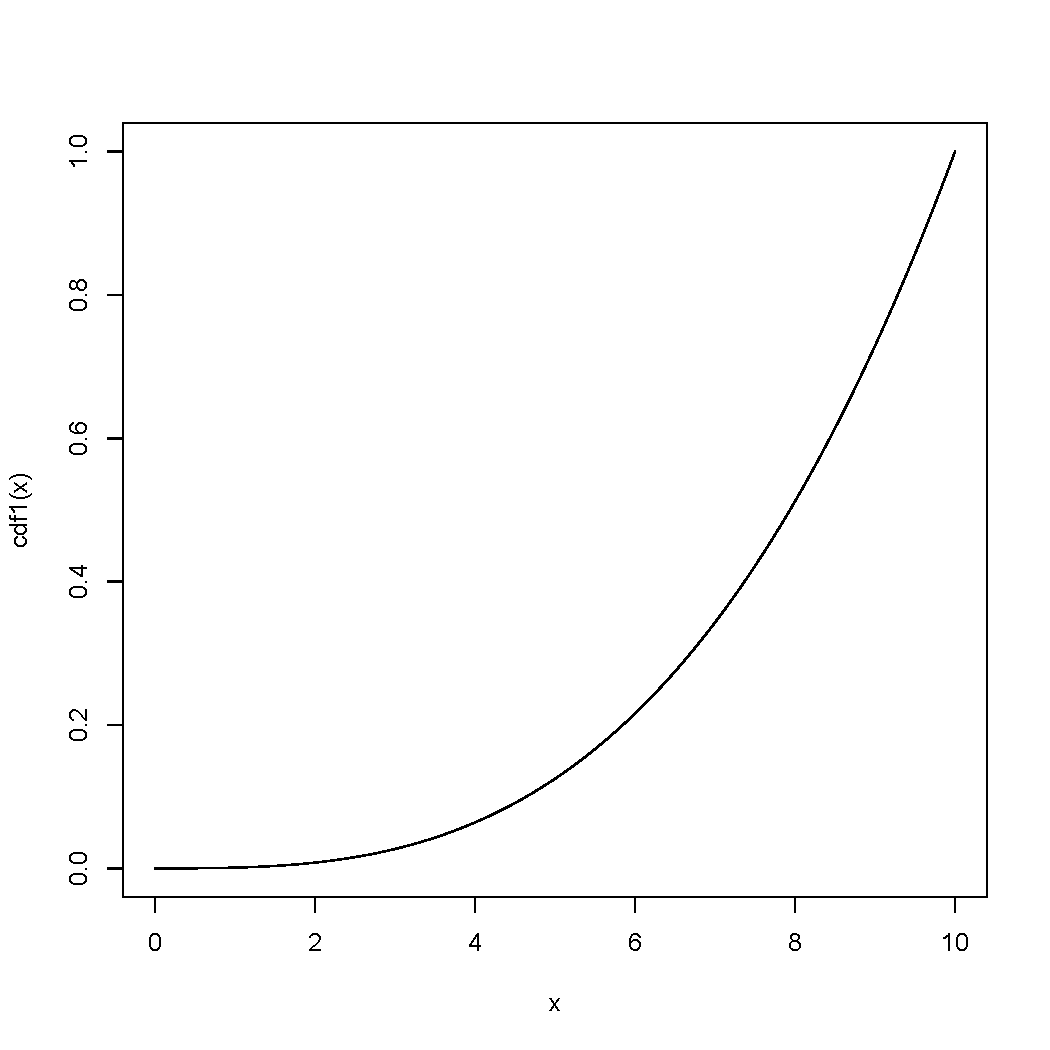
\includegraphics[width=3in]{CDF1.pdf}



\end{enumerate}
\pagebreak
\item A median is a value m such that $P (X \leq m) \geq 1/2$ and $P (X \geq m) \geq 1/2$. If $X$ is continuous, $m$ satisfies  $\int_{-\infty}^m f (x)dx = \int_m^{\infty} f(x)dx = 1/2$. Find the median for
\begin{enumerate}
\item Uniform(a, b) distribution.  
\item[A)]$\int_{a}^m \frac{1}{b-a}dx= \frac{m-a}{b-a}=1/2$ so $m-a=\frac{b-a}{2}$ and $m=\frac{b+a}{2}$



\item Exponential($\lambda$) distribution $f(x)=\lambda e^{-\lambda x}$.\
\item[A)]$\int_{-\infty}^m \lambda e^{-\lambda x}dx=1/2$  So $e^{-\lambda m}=1/2$ and solving for m gives us $m=\frac{log(1/2)}{-\lambda}=\frac{-log(2)}{-\lambda}=\frac{log(2)}{\lambda}$
\end{enumerate}
\end{enumerate}

\item \textsc{Calculating things}
\begin{enumerate}[1)]
\item You receive survey data for N people which includes two pieces of information: variable X and variable Y for each individual. You calculate the following functions of the data,
$$\mu_X=4$$
$$\mu_Y=2$$
$$\mu_{XY}=12$$
$$\sigma_X^2=8$$
$$\sigma_Y^2=4$$
What is the correlation between X and Y?  $\frac{12-4*2}{\sqrt{8}*\sqrt{4}}=\frac{1}{\sqrt{2}}$
\item An insurance company believes that people can be divided into two classes: those who are accident prone and those who are not. The statistics show that an accident-prone person will have an accident at some time with probability 0.4, whereas the probability decreases to 0.2 for a non-accident-prone person. The company also believes that 30\% of the population is accident prone.

\begin{enumerate}[a)]
\item What is the probability that a new policyholder will have an accident within a year of purchasing a policy?
P(accident)=P(accident$|$prone)*P(prone)+P(accident$|$not prone)*P(not prone)=.4*.3+.2*.7=.26
\item  Suppose that a new policyholder has an accident within a year of purchasing a policy: what is the probability that s/he is accident-prone?

P(prone$|$accident)=P(accident$|$prone)*P(prone)/(P(accident)= (.4*.3)/.26=.46

\end{enumerate}

\end{enumerate}
\item \textsc{Inference} 
\begin{enumerate}

\item Some one gives you an estimated proportion of $.6$ supporting Trump (versus Clinton) based on a poll. He also says the variance of the estimate is .0024.
\begin{enumerate}
\item[a)]  He forgot to tell you the sample size; what is it?  $p*(1-p)/n=.0024$, so $n=.24/.0024=100$
\item[b)] Comment on the plausibility of the hypothesis that Trump has same level support as Clinton in the population.  A reasonable test statistic is $(.6-.5)/\sqrt{.0024}=2.041$, which is according to the normal distribution, only likely to occur in 4 percent of cases (considering both tails) if the true level of support was 0.5.

\end{enumerate}
\item  In a simple random sample of 1,000 citizens, 560 oppose a public health care option and 440 support. Is it reasonable to assume that the country is evenly divided on this question? $(.56-.5)/\sqrt{.44*.56/1000}=3.8$, which strongly suggests that the nation is not evenly divided.

\item Suppose $\bar{X}$ is the sample mean of 90 observations from a population with mean $\mu$ and variance $\sigma^2$.  Find 95\% confidence limits for $\bar{X}$.
\begin{enumerate}
\item[a)] Using Chebychev.  
$$P(|\bar{X}-E(X)|\geq c )\leq \frac{\sigma^2_{\bar{x}}}{c^2}$$

Choosing $c=\sigma_{\bar{x}}k$, we get the following:

$$P(|\bar{X}-E(X)|\geq k\sigma_{\bar{x}} )\leq \frac{1}{k^2}$$
so $.05=\frac{1}{k^2}$, $k=4.47$
$$P(|\bar{X}-E(X)|\geq 4.47\sigma/\sqrt{90} )\leq .05$$
$$P(E(X)-4.47\sigma/\sqrt{90} \geq \bar{X}\geq E(X)+4.47\sigma/\sqrt{90})\leq .05$$

The confidence interval is + and - $.47\sigma$

\item[b)] Using Central Limit Theorem.
$$P(\frac{|\bar{X}-E(X)|}{\sigma/\sqrt{90}}|\geq \Phi^{-1}(.025))=.05$$
$$P(|\bar{X}-E(X)|\geq 1.96\sigma/\sqrt{90})=.05$$

The confidence interval is + and - $.2\sigma$.

\item[c)] Compare the two limits.  
\item[A)] It is less than half as wide when we have the central limit theorem.

\end{enumerate}

\end{enumerate}
\end{enumerate}
\end{document}

